\documentclass[a4paper,twocolumn]{article}

\newcommand{\itwoc}{I$^2$C }
\usepackage{graphicx}
\graphicspath{{./images/}}
\title{Student Robotics 2009\\ Peripheral Interconnect}

\begin{document}
\maketitle

All the Student Robotics boards are provided with regulated power for logic circuits and a data connection through the ``RJ11 cables''\footnote{The connectors on the ends of the cables are not necessarily RJ11 connectors.  The naming of these connectors has not been standardised.  It \emph{seems} that the connectors referred to as RJ11 here are most commonly referred to as 4P4C, RJ9, RJ10 or RJ22.}, which are 4-core cables terminated in 4P4C connectors, shown in figure~\ref{fig:coil}.

The pinout of the 4P4C connector is shown in Table~\ref{tab:4p4c-pinout}.  The socket pin numbering is shown in figure~\ref{fig:4p4c-pin-num}.  The RJ11 cables are wired so that two sockets connected together with one have the same signal on numerically identical pins.

Two sockets connected by an RJ11 cable have the same signal on similarly numbered pins (for example pin 1 on the motor board's 4P4C connector connects to pin 1 on a 4P4C connector on the power board).

\begin{figure}
  \begin{center}
    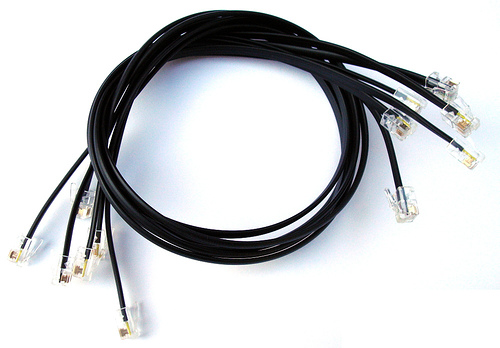
\includegraphics[width=5cm]{./images/coil.jpg}
  \end{center}
  \caption{\label{fig:coil}Cables supplied in SR kit.}
\end{figure}

\begin{table}
  \caption{\label{tab:4p4c-pinout}4P4C Pinout}

  \begin{center}
    \begin{tabular}{|c|c|c|}
      \hline
      \textbf{Pin} & \textbf{Name} & \textbf{Description} \\
      \hline
      1 & VDD & 3.3V logic power rail\\
      2 & SDA & \itwoc data \\
      3 & VSS & Ground \\
      4 & SCL & \itwoc clock\\
      \hline
    \end{tabular}
  \end{center}
\end{table}


\begin{figure}
  \begin{center}
    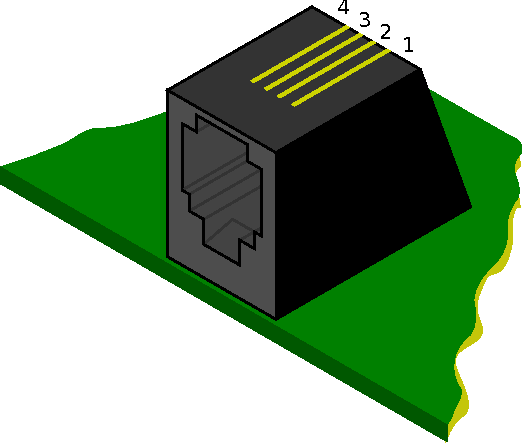
\includegraphics[width=6.5cm]{./images/4p4c.pdf}
  \end{center}
  \caption{\label{fig:4p4c-pin-num}4P4C Pin Numbering}
\end{figure}



\end{document}